% !TEX spellcheck = en_US
% !TeX program = pdflatex
% !TeX TXS-program:bibliography = txs:///bibtex
% !BIB program = bibtex

%% LMU-MI-HS-Template
%% This template is an adaptation of the IEEE InfoVis/Vis format
%% http://www.cs.sfu.ca/~vis/Tasks/camera_tvcg.html
%% Last update: Bastian Pfleging, 05.2016

\documentclass[journal]{vgtc}                % final (journal style)
\usepackage[english]{babel}
\usepackage{mathptmx}
\usepackage{graphicx}
\usepackage{times}
\usepackage[hyphens]{url}
\usepackage{float}

\usepackage[backend=bibtex, style=numeric, isbn=true, doi=true, maxnames=99]{biblatex}
\addbibresource{literature.bib}

\DeclareGraphicsExtensions{.pdf,.jpg,.pdf,.mps,.png}
\graphicspath{{img/}} 


\normalfont


%% Paper title.

\title{Intimate data in Personal Informatics: Tracking, sharing and personal boundaries?}

%% Put your name here
\author{Diana Irmscher}
\authorfooter{
%% change name, course (Media Informatics/Informatics/etc) and email for the footer
\item
  Diana Irmscher is studying Media Informatics at the University of Munich, Germany, E-mail: d.irmscher@campus.lmu.de
\item
  This research paper was written for the Media Informatics Advanced Seminar 'Advanced Seminar in Media Informatics',
  2018
}


%% Abstract section.
\abstract{
Sum up your work and the ideas behind it in 150 to 250 words.
} % end of abstract

%% Keywords that describe your work.
\keywords{Fill, In, Your, Own, Keywords}

%%%%%%%%%%%%%%%%%%%%%%%%%%%%%%%%%%%%%%%%%%%%%%%%%%%%%%%%%%%%%%%%
%%%%%%%%%%%%%%%%%%%%%% START OF THE PAPER %%%%%%%%%%%%%%%%%%%%%%
%%%%%%%%%%%%%%%%%%%%%%%%%%%%%%%%%%%%%%%%%%%%%%%%%%%%%%%%%%%%%%%%%

\begin{document}

\firstsection{Problem Statement}

\maketitle

% ------------------------------------------------------------------------------
%
% This is only an exemplary structure for your paper! Feel free to change the names of the sections
% and subsections! 
%
% ------------------------------------------------------------------------------

This is where your introductory text starts. As this should be a scientific publications, do not forget to cite other scientific papers to justify your argumentation. You might mention the work of Cooper et al.~\cite{Cooper2006}, a paper on the effects of 2D geometric transformation on visual memory~\cite{Lam2006}. If LaTeX displays only question marks \cite{IWonderIfThisSourceExists2013} and shows warnings, re-run the build process. If that does not fix it, check your source name for typos. References to web pages should be placed in footnotes\footnote{\url{http://www.mckinsey.com/industries/automotive-and-assembly/our-insights/ten-ways-autonomous-driving-could-redefine-the-automotive-world}, \newline all URLs last accessed 2016-05-30}. It is sufficient if the access date is only mentioned for the first link as shown before.

\section{Introduction}

\section{Related Work}

\subsection{Justification}

\subsection{Evaluation}

\section{Research Plan}

\begin{table}
  %% Table captions on top in journal version
  \caption{Research Plan}
  \label{tab:vis_accept}
  \scriptsize
  \begin{center}
    \begin{tabular}{ll}
      Date & Objective \\
    \hline
      16.04.2018 &  First Meeting  with supervisors, prepare proposal \\
      20.04.2018 & Submit final proposal \\
      08.05.2018 & Submission of first paper draft \\
      11.05.2018 & Submission of 60 sec. presentation \\
      29.05 Sub
	\end{tabular}
  \end{center}
\end{table}


\section{Risk Analysis}

\begin{table}
%% Table captions on top in journal version
  \caption{Vis Paper Acceptance Rate}
  \label{tab:vis_accept}
  \scriptsize
  \begin{center}
    \begin{tabular}{cccc}
      Year & Submitted & Accepted & Accepted (\%)\\
    \hline
      1994 &  91 & 41 & 45.1\\
      1995 & 102 & 41 & 40.2\\
      1996 & 101 & 43 & 42.6\\
      1997 & 117 & 44 & 37.6\\
      1998 & 118 & 50 & 42.4\\
      1999 & 129 & 47 & 36.4\\
      2000 & 151 & 52 & 34.4\\
      2001 & 152 & 51 & 33.6\\
      2002 & 172 & 58 & 33.7\\
      2003 & 192 & 63 & 32.8\\
      2004 & 167 & 46 & 27.6\\
      2005 & 268 & 88 & 32.8\\
      2006 & 228 & 63 & 27.6
    \end{tabular}
  \end{center}
\end{table}

Here is a sample illustration. Again, do not forget to mention it somewhere in your text \textit{(see figure \ref{fig:sampleimage})}.
\begin{figure}[htb]
  \centering
  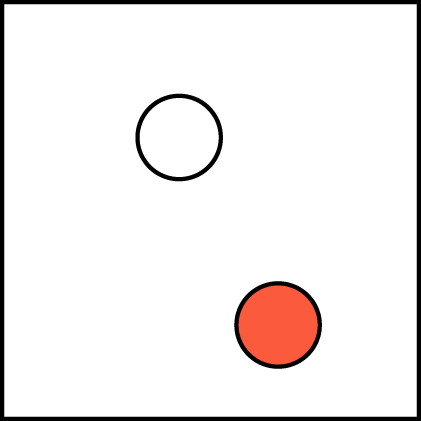
\includegraphics[width=1.5in]{sample}
  \caption{Sample illustration.}
  \label{fig:sampleimage}
\end{figure}

%% Do not change the following:
%\bibliographystyle{abbrv}
\printbibliography
\end{document}
